\section{Networks}\label{chap:networksBasics}
contents: Basics of netowrks: Adjacency matrix, directed/indirected graphs, 

purpose: nobody knows


To understand the spreading of disease of networks, it is necessary to have a basic understanding of networks and their behavior. The following chapter is going to focus on the theory of networks and give some insights on other interesting topics.
\subsection{Network Basics}
The mathematical representation of a network is a graph, a schematically drawing of such a construct is shown in figure \ref{fig:simpleNetwork}. The so called graph theory is a branch of mathematics which studies graphs, which are made up of nodes and edges (or links), the connections between the nodes. In our case the different nodes are farms and the links are occurring trades between those farms.
\paragraph{Adjacency Matrix}
In order to describe the links between the nodes, the so called adjacency matrix is being used. Following \citep{BAR16} it's entries $a_{ij}$ are either one or zero depending on the existence of a link from node $j$ to node $i$. Note that this contradicts the convention of graph theory where the entries $a_{ij}$ of the adjacency matrix are 1, if there is an edge from node $i$ to node $j$.
\begin{figure}[htbp]
\centering
\noindent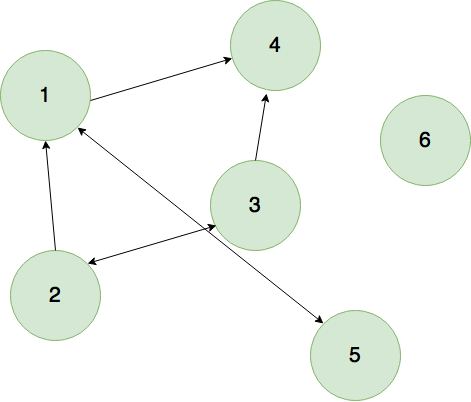
\includegraphics[width=0.4\linewidth,height=\textheight,
keepaspectratio]{Graph.png} 
\caption[Graph Example]{The picture shows  a simple example of a network with 6 Nodes. The arrows are showing the connections (links) between the different nodes. Some of the links are unidirectional, others bidirectional.}
\label{fig:simpleNetwork}
\end{figure}
Following this concept the adjacency matrix for the network in figure \ref{fig:simpleNetwork} looks as follows:
\begin{equation}
A = \left( \begin{matrix}
 1 & 0 & 0 & 1 & 1 & 0\\
 1 & 1 & 1 & 0 & 0 & 0\\
 0 & 1 & 1 & 1 & 0 & 0\\
 0 & 0 & 0 & 1 & 0 & 0\\
 1 & 0 & 0 & 0 & 1 & 0\\
 0 & 0 & 0 & 0 & 0 & 1
 \end{matrix}
 \right). \label{eq:adjMatExamp}
\end{equation}
Note that the entries $a_{ii}$ of $A$ are always $1$ (every node is connected to itself) and that the matrix would be symmetric if all links were bidirectional. 
If certain links were stronger then others, one would attach so called weights to the vertices. If the link represented by $a_{rs}$ had the strength (or weight) $85$, this would be represented by $a_{rs}= 85$. 
\paragraph{Reachability}
One way of determining if node $k$ is reachable by node $l$ in $n$ steps is taking the $n$th power of $A$ and inspecting it's entry $a_{nl}$. For example the 3rd power of matrix \ref{eq:adjMatExamp} would show that all nodes but nodes 6 are reachable by node 3 within 3 steps. If one would want to calculate all nodes that could be reached within $N$ or less steps, one would have to take the sum:
\begin{equation}
K_N = \sum_{n=0}^N A^n, \label{eq:reachability}
\end{equation}
with the reachability matrix $K_N$.
\paragraph{Disease Spread On Networks}
As shown in picture \ref{fig:disSpreadExampl}, a given disease can spread from one node to another in case there is a link between them. For example the disease can spread from node 3 to nodes 4 and 2 in the first time step. Node 1 will soon thereafter be infected by node 2, but not by node 4. If the structure of the network stays the same, node 6 will never be infected.
\begin{figure}[htbp]

\begin{minipage}{0.5\textwidth}
\centering
\noindent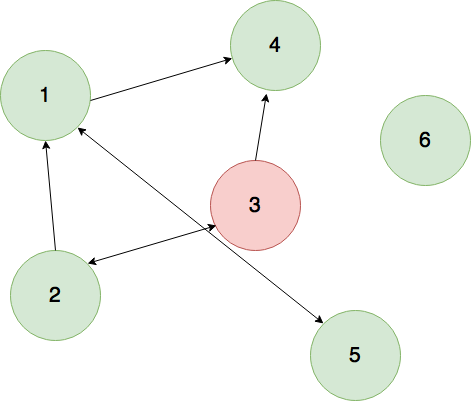
\includegraphics[width=0.9\linewidth,height=\textheight,
keepaspectratio]{Graph2.png} 
\end{minipage}
\begin{minipage}{0.5\textwidth}
\centering
\noindent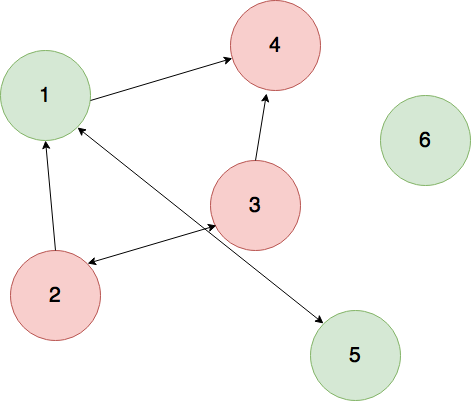
\includegraphics[width=0.9\linewidth,height=\textheight,
keepaspectratio]{Graph3.png} 
\end{minipage}
\caption[Infection Spread On A Static Network]{This picture shows the spread of a disease along the links between the nodes. Red nodes are infected, green ones are still susceptible. The third node is infected first. Nodes 4 and 2 get infected after time step 1.}
\label{fig:disSpreadExampl}
\end{figure}

\paragraph{Disease Spread On Time Dependant Networks.}
When it comes to applications for the basics discussed above, one has to find networks in real life. Unfortunately most networks in real life are not as simple and static as the examples shown above. 
If the networks changes it's structure over time, the adjacency matrix becomes time dependant:
\begin{equation}
A = A(t).
\end{equation}
This implies that the reachability in a time dependant network also changes over time and therefore depends on the start time:
\begin{equation}
K(t,t_0) = \sum_{}^{}\prod_{n=t_0}^{t}A(n)
\end{equation}
Picture \ref{fig:timeDependantNetworkSpread} illustrates this. The network only changes slightly but makes it impossible for the disease to spread from node 1 to node 5. Instead it infects node 6 which would have stayed unaffected if the network would have stayed in it's earlier state. Even if the network would go back to it's earlier configuration the disease would not spread from node 1 to node 5 because node 1 will already have recovered in the next time step and therefore be unable to infect any other node. The only possibility for the disease to reach node 5 would be an upcoming link from node 6 to node 5.

\begin{figure}[htbp]
\begin{minipage}{0.5\textwidth}
\centering
\noindent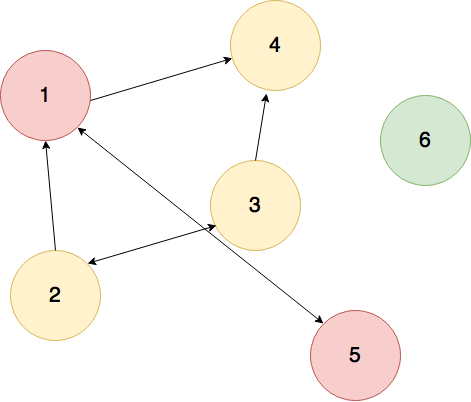
\includegraphics[width=0.9\linewidth,height=\textheight,
keepaspectratio]{Graph4.png} 
\end{minipage}
\begin{minipage}{0.5\textwidth}
\centering
\noindent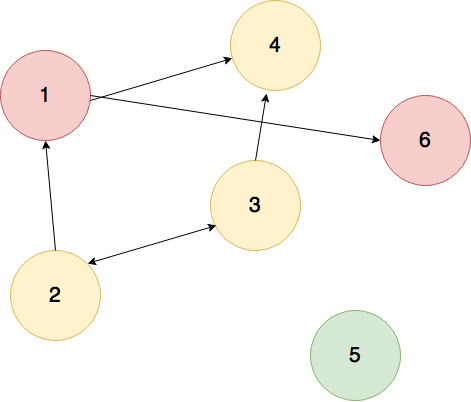
\includegraphics[width=0.9\linewidth,height=\textheight,
keepaspectratio]{Graph5.png} 
\end{minipage}
\caption[Disease Spread On A Time Dependant Network]{The two graphs show the difference a time varying network can make for the spread of a disease on it. In the left hand picture node 1 infects node 5. In the picture on the right hand side node 1 infects node 6 instead. Even if the network would go back to it's earlier state, node 1 would be recovered (yellow) in the next time step and therefore be unable to infect node 5. Note that node 4 can not be infected by node 1 anymore because it had been infected earlier and became recovered and therefore immune in the mean time.}
\label{fig:timeDependantNetworkSpread}
\end{figure}


\subsection{Networks Of Stochastic Oscillators}
It is possible to analytically predict the behavior of a whole system of many nodes with a basic SIR-Model, as it was shown by \citep{ROZ11}. The system described by them was a network of $n$ cities which exposed a fix point. In contrast to the examples given above this means that the node is not either infected or susceptible as a whole, but every node is split up into different compartments. There is a probability for an individual to travel from one city to another. This leads to a statistical oscillating system. The fluctuations in the system could be described by a power spectrum derived from a Fokker-Planck equation. 
The eigenvalues of the system turn out to be quite close to the eigenvalues of a single city. The phenomenological explanation for this is that the cities behave like a single city, if the coupling and therefore the mixing is pretty strong. They behave like single cities, if the coupling is weak. 
Transferring this result on the case of BVD would imply that the stable state of the whole system would be close to the stable state of a single farm. The distributions for single farms can be found in chapter \ref{chap:rlDataRegulationGermany}. However these results require a network which allows for all farms to at least get infected once. Therefore it might not be applicable to our network since some farms don't necessarily buy cows.